%% ===================================================================
%% Appendix F. Detailed Experimental Results and Reproducibility
%% Per-dataset tables and breakdowns behind sec:experiments, the
%% fraud-detector walk-through, and the reproducibility note. Adds the
%% two verified orphan figures (fig_attack_comparison, fig_positioning).
%% Labels app:experiments / app:attack_full / app:baselines /
%% app:smoothing / app:phase_scal / app:ablations / app:explicit /
%% app:fraud / app:repro and the table/figure labels are preserved.
%% ===================================================================
\section{Detailed Experimental Results}
\label{app:experiments}

This section gives the detailed tables and per-dataset breakdowns behind the headline numbers of
\cref{sec:experiments}, followed by the fraud-detector walk-through and the reproducibility note. All
results use the 10 fixed seeds of \cref{app:repro}.

\subsection{Four-Quadrant Attack Comparison}
\label{app:attack_full}
\Cref{tab:attack_full} evaluates \AEGIS across the four quadrants of (gradient-based, gradient-free)
$\times$ (equilibrium-shift, classification-loss). The SVD direction maximizes first-order equilibrium
shift by construction (\cref{prop:attack}); what matters is non-circularity and cost. A transfer
direction from a separately trained surrogate (zero shared gradients) recovers $99\%$ of the one-query
damage ($\cos{=}0.99$), versus $44{\pm}4\%$ for a $512$-query black-box search, so the fault line is
model-intrinsic rather than a gradient artifact. Per query it delivers $74$--$156\times$ the damage of a
$50$-step PGD~\cite{madry2018towards}; classification-loss PGD inflicts $15$--$70\%$ less at $50\times$
the cost, IFT-gradient PGD (solver validation, not an independent baseline) $72$--$92\%$, and prediction
flips stay $0$--$1.8\%$ for all methods. \Cref{fig:attack_comparison} visualizes the equilibrium-damage
column.

\begin{figure}[t]
\centering
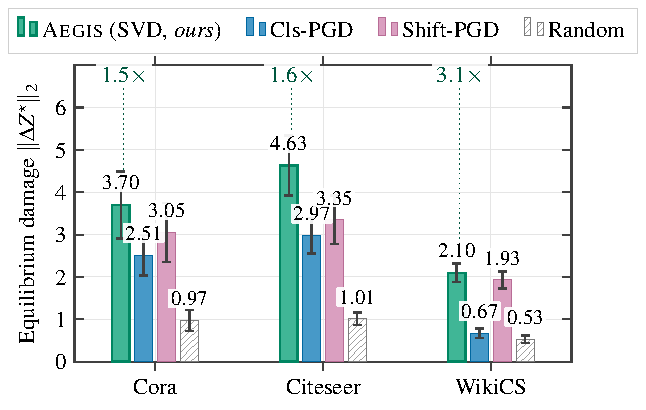
\includegraphics[width=\columnwidth]{figures/fig_attack_comparison.pdf}
\caption{Equilibrium damage $\norm{\Delta Z^\star}_2$ at $\varepsilon{=}0.10$ across 10 seeds, for the
one-query \AEGIS (SVD) attack against classification-loss PGD, IFT-gradient (shift) PGD, and a random
baseline, on Cora, Citeseer, and WikiCS. Visual companion to \cref{tab:attack_full}: one analytic
\AEGIS query inflicts $1.5$--$3.1\times$ the damage of a $50$-step Cls-PGD run per dataset, at a fraction
of its cost.}
\label{fig:attack_comparison}
\end{figure}

\textbf{Radius vs.\ smoothing.} Randomized smoothing~\cite{bojchevski2020efficient} gives constant
per-node base radii ($0.123$ vs.\ \AEGIS's $0.078$ at $\sigma{=}0.05$), and localized
smoothing~\cite{schuchardt2023localized} needs ${\sim}10^5$ MC samples per node; both lack edge
structure. \AEGIS radii are instead structurally informative ($r_v{\approx}0.10$ in dense regions,
$0.01$ at boundaries), a complementary point on the certificate-versus-diagnostic frontier.

\textbf{Classification-gradient edges differ.} Per-edge classification gradients anti-correlate with
discrete ground truth on Cora ($\tau{=}\ms{-0.20}{0.05}$ vs.\ \AEGIS's $\ms{+0.32}{0.04}$) and stay near
zero elsewhere; \AEGIS achieves $2$--$6\times$ higher P@10, confirming that equilibrium and
classification sensitivities are distinct vulnerability surfaces. Per-edge finite differences reproduce
the $S_c$ column-norm ranking ($\tau{=}0.999$), and iterative $S_c$ recomputation closes $\le3$\,pp of
the static-versus-greedy gap, so the static ranking is the headline. The four-quadrant
equilibrium-damage table itself is promoted to the main text (\cref{tab:attack_full},
\cref{sec:audit}); the per-edge analyses here are the supporting detail.

\subsection{Comparison with Prior Structural Baselines}
\label{app:baselines}
\Cref{tab:baselines} reports head-to-head numbers against the GR-BCD and PR-BCD structural
attackers~\cite{geisler2021robustness}. \AEGIS is a label-free one-query proxy; the question is how much
of each gold-standard signal it retains. GR-BCD aligns with $S_c$ on Pubmed ($\tau{=}{+}0.69$) but
decorrelates on Cora ($\tau{=}{+}0.16$); the budgets shown ($k{\le}10$) are \AEGIS's early-warning
regime, where its one-pass diagnostic is competitive, while GR-BCD/PR-BCD dominate raw damage at the
high budgets they target. AGNNCert~\cite{li2025agnncert} is a sound certificate against a bounded
\emph{number} of discrete edge edits (a majority vote over hash-partitioned sub-graphs), whereas
\AEGIS's $r_v$ bounds a \emph{continuous} edge-weight budget $\norm{\delta\Ahat}_F$; the two target
different threat models and are complementary rather than comparable on one radius axis. \AEGIS also
beats degree-proportional, edge-betweenness, and spectral rankings at $\varepsilon{=}0.01$
($+6$--$148\%$ AtkAdv, Wilcoxon $p{<}0.001$) and inflicts $3$--$10\times$ more equilibrium damage than
Mettack~\cite{zugner2019adversarial} in the early-warning regime $k\!\in\!\{1,\ldots,5\}$
($\mathbf{149/150}$ paired wins, $p{<}10^{-43}$).

\Cref{fig:positioning} positions these threads on a seven-axis capability radar, each polygon tracing
the \emph{frontier} of its thread (the best any cited method in it achieves on that axis). No single
method covers every axis: structural attacks own attack direction, per-edge ranking, and large-budget
damage; the white-box gradient is the attribution oracle that \AEGIS only proxies
($\tau{=}0.16$--$0.99$), while certifiers own the per-node certificate. \AEGIS wins no specialist axis
outright, but spans all seven, reading an attack direction, per-edge
attribution, and a first-order per-node certificate off a single closed-form, label-free $S_c$ query on
an off-the-shelf model. Its third pillar, hardening via the $\sigma_1(S_c)$ penalty of
\cref{sec:defense}, is a different kind of claim, benchmarked there against the robust-architecture
thread rather than scored on this audit-and-certify radar.

Among the certifiers it scores, AGNNCert~\citep{li2025agnncert} is deterministic ($T{=}30$--$80$ subgraph evaluations) and localized smoothing~\citep{schuchardt2023localized} is a \emph{collective} certificate at ${\sim}10^5$ samples/node; both require specialised retraining and name no vulnerability-driving edges.

\begin{table}[t]
\centering
\caption{\AEGIS vs.\ external baselines (10 seeds). GR-BCD~\cite{geisler2021robustness} is the
BCD-family scalable structural attacker (PR-BCD is the same paper's larger-budget variant, see text).}
\label{tab:baselines}
\footnotesize
\setlength{\tabcolsep}{3pt}
\begin{tabular*}{\columnwidth}{@{\extracolsep{\fill}}l l c c r@{}}
\toprule
Baseline & Setting & \AEGIS & Baseline & $\tau$ \\
\midrule
GR-BCD & Pubmed $k{=}10$ & $0.356$ & $0.350$ & $\mathbf{+0.69}$ \\
GR-BCD & Cora $k{=}5$ & $0.643$ & $1.207$ & $+0.16$ \\
\bottomrule
\end{tabular*}
\end{table}

\subsection{Certification vs Randomized Smoothing}
\label{app:smoothing}
The matched smoothing $\sigma{=}\varepsilon/\sqrt{2|E|}$ (Frobenius ball) is so small that the smoothed
classifier is unchanged and abstains; only on the strictly larger per-coordinate ball
($\sigma{=}\varepsilon$) does it certify ($0.77$--$0.96$ of nodes), and then at
$\mathbf{23{,}000}$--$\mathbf{57{,}000}\times$ the wall-clock of the zero-sample $S_c$ bound. Even on the
matched ball the analytic certificate is non-vacuous and $\mathbf{11{,}700}$--$\mathbf{16{,}700}\times$
faster: the comparison favors smoothing twice (larger ball, best matching), yet the certificate of
\cref{tab:smoothing} dominates by four orders of magnitude.

\subsection{Phase Transition and Scalability}
\label{app:phase_scal}
\textbf{Phase transition.} \Cref{fig:phase_transition} sweeps $\kappa_{\max}{\in}[0.30,0.99]$ on Cora
(10 seeds). Even when the spectral-normalization cap is pushed to $0.99$, driving the theoretical
$\ecrit$ down $230\times$, the trained ReLU pattern keeps $\rho(J_z)\le0.42$, so the resolvent grows
only $\mathbf{1.17{\to}1.80}$. This is a $\mathbf{2}$--$\mathbf{4\times}$ spectral-radius margin to
criticality ($\rho{=}1$), the operative quantity behind $\ecrit$, stable across the sweep. Training
converges throughout, and the matrix-free pipeline reaches its 50-step fixed-point budget at
$\kappa_{\max}{\ge}0.85$.

\begin{figure*}[t]
\centering
\begin{minipage}[t]{0.33\textwidth}
\centering
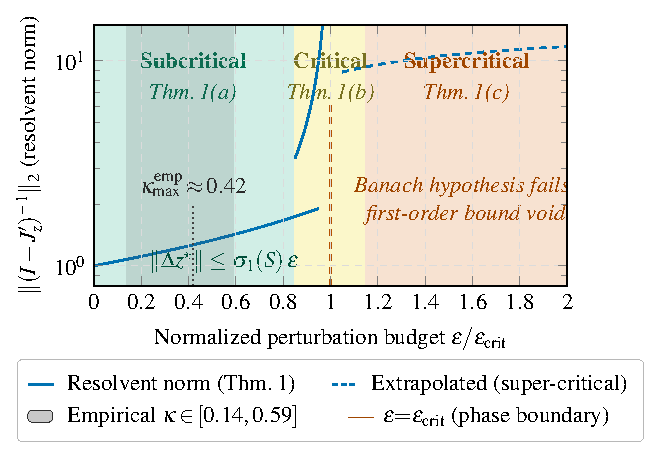
\includegraphics[width=\linewidth]{figures/fig_phase_transition.pdf}
\caption{Three-regime characterization of \cref{thm:phase_transition}. The empirical $\kappa$ band
(grey) saturates well below the spectral-normalization ceiling, so the empirical resolvent growth is far
milder than the worst-case $1/(1-\kappa)$ divergence at $\varepsilon\to\ecrit$.}
\label{fig:phase_transition}
\end{minipage}\hfill
\begin{minipage}[t]{0.655\textwidth}
\centering
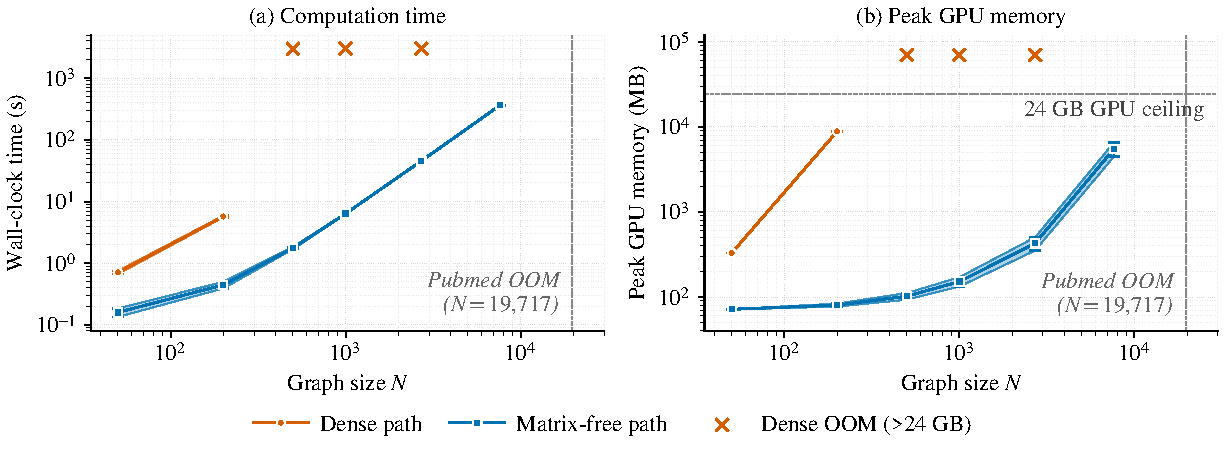
\includegraphics[width=\linewidth]{figures/fig_scalability.pdf}
\caption{Dense vs.\ matrix-free \AEGIS pipeline (RTX 4090). The dense path scales as $O((Nd)^3)$,
exceeding $24$\,GB beyond $N{=}200$; the matrix-free path is roughly $O(N\log N)$ in time and sub-linear
in memory, reaching Amazon Photo ($N{=}7{,}650$) at $365$\,s and $5.5$\,GB.}
\label{fig:scalability}
\end{minipage}
\end{figure*}

\textbf{Scalability and matrix-free self-consistency.} \Cref{fig:scalability} compares the dense and
matrix-free pipelines. The matrix-free $S_c v$ implements the dense $S_c$ up to Neumann truncation;
$\sigma_1$ agrees within $0.03\%$ at $N{=}200$ (per-edge $\tau{=}0.999$), and the analytic truncation
residual $\kappa^{200}\in[10^{-105},10^{-48}]$ across the suite (\cref{eq:neumann-tail}). For larger $N$
the rSVD error~\cite{halko2011finding} is bounded by the spectral gap; Pubmed ($N{=}19{,}717$) exceeds
$24$\,GB on the dense path.

\subsection{Ablations and Defense}
\label{app:ablations}
\textbf{Subgraph size.} Varying $N{\in}\{30,50,100,200\}$ on Cora (10 seeds), tightness is stable at
$1.01$--$1.02$ for $N{\le}100$ and degrades to $1.031$ at $N{=}200$; we use $N{=}50$ by default
($66\times$ faster). \textbf{Full-graph scale.} A 50-node BFS covers only ${\sim}1.8\%$ of a citation
graph's edges (Cora $\tau{=}0.16$), so at this scale we run \AEGIS on the full graph, where its edge
advantage over degree-proportional ranking \emph{amplifies} to $\mathbf{9.82\times}$ (Citeseer) and
$\mathbf{3.25\times}$ (Cora) at $k{=}10$, against ${\approx}1.1\times$ on subgraphs.
\textbf{Hyperparameters.} Tightness is stable across $d{\in}\{16,32,64,128\}$; the spectral-norm ceiling
$c{\in}\{0.5,0.9\}$ traces the accuracy--robustness frontier ($r_v{=}0.147$ at $72.1\%$ vs.\ $0.089$ at
$80.6\%$).

\textbf{Edge protection and the delocalization of vulnerability.} On the full graph (Cora, $N{=}2{,}708$,
10 seeds), masking the top-$k$ edges by $v_{ij}$ cuts $\sigma_1(S_c)$ damage by $2.4{\pm}1.8\%$ at
$k{=}5$ and $4.6{\pm}2.9\%$ at $k{=}10$, a $\mathbf{12}$--$\mathbf{46\times}$ gain over random masking but
far below the $42$--$61\%$ a 50-node subgraph reports (where $k{=}5$ is already $10\%$ of its edges). The
reason is structural: the leading attack mode is \emph{delocalized} (participation ratio $41$--$89$
edges), so removing a handful excises a negligible slice. Reaching subgraph-scale reduction needs
$2$--$8\%$ of edges masked, and adaptive recomputation erodes the gain a further $1$--$2$\,pp. \AEGIS
therefore \emph{localizes} risk for attribution and triage rather than yielding a few-edge defense, the
failure mode that sober-look critiques~\cite{mujkanovic2022defenses} flag.

\subsection{Per-Architecture Characterization (Explicit GNNs)}
\label{app:explicit}
For $K$-layer explicit GNNs (GCN, SAGE, GIN, APPNP,
GAT$^\dagger$~\cite{kipf2017semi,hamilton2017inductive,xu2019how,klicpera2019predict,velickovic2018graph})
we form $S_K{=}\partial\mathrm{vec}(Z_K)/\partial\mathrm{vec}(A)$ by finite differences and build $S_c$
from $S_K$ identically (\cref{prop:explicit}). \Cref{tab:explicit} reports the per-architecture
characterization on Cora: IGNN carries \cref{thm:phase_transition}, while the explicit models receive
the computational tool without the regime characterization.

\begin{table}[t]
\centering
\caption{$S_c$ framework on 7 GNN architectures (Cora, 10 seeds). Tight.: actual/predicted shift ratio.
AtkAdv: \AEGIS/random damage. $\tau$: Kendall of the \emph{unweighted} $v_{ij}$ ranking vs.\ single-edge
removal; the edge-weighted $A_{ij}v_{ij}$ ranking of \cref{prop:transfer} (\cref{fig:tau_heatmap}) is the
higher headline score. Acc: full-graph test accuracy.}
\label{tab:explicit}
\small
\begin{tabular*}{\columnwidth}{@{\extracolsep{\fill}}l rrrr@{}}
\toprule
Model & Tight. & AtkAdv & $\tau$ & Acc \\
\midrule
IGNN (eq.) & $\ms{1.01}{.00}$ & $\ms{7.6}{0.5}\times$ & $\ms{+.32}{.04}$ & $\ms{77.5}{1.7}$ \\
\midrule
GCN-2 & $\ms{1.00}{.00}$ & $\ms{3.6}{0.6}\times$ & $\ms{-.04}{.03}$ & $\ms{78.9}{0.9}$ \\
GCN-4 & $\ms{1.02}{.00}$ & $\ms{3.4}{0.4}\times$ & $\ms{+.49}{.02}$ & $\ms{78.3}{1.8}$ \\
GIN-2 & $\ms{1.01}{.00}$ & $\ms{2.6}{0.1}\times$ & $\ms{+.33}{.03}$ & $\ms{76.6}{1.9}$ \\
GAT$^\dagger$ & $\ms{1.01}{.01}$ & $\ms{2.1}{0.1}\times$ & $\ms{\mathbf{+.54}}{.06}$ & $\ms{77.8}{1.2}$ \\
SAGE-2 & $\ms{1.00}{.00}$ & $\ms{1.9}{0.2}\times$ & $\ms{+.22}{.10}$ & $\ms{77.5}{1.5}$ \\
APPNP & $\ms{1.02}{.00}$ & $\ms{3.4}{0.3}\times$ & $\ms{+.35}{.01}$ & $\ms{\mathbf{82.2}}{0.6}$ \\
\bottomrule
\end{tabular*}
\end{table}

\textbf{GAT$^\dagger$ scope.} Standard GAT uses $A$ as a binary mask, so $\partial Z/\partial A_{ij}{=}0$
on existing edges and $S_c$ is undefined; our GAT$^\dagger$ modulates attention by the edge weight
($h_i'=\sum_j\Ahat_{ij}\alpha_{ij}Wh_j$), restoring differentiability and yielding tightness $0.99$,
AtkAdv $4.4\times$, $\tau{=}{+}0.36$. Binary-mask architectures (hard attention, max/min aggregation,
GATv2~\cite{brody2022how}-style dynamic-attention masking) fall outside the framework. \textbf{Robust
backbones.} Under the $\sigma_1(W){\le}0.9$ cap, RobustGCN-lite~\cite{zhu2019robust} and
GNNGuard-lite~\cite{zhang2020gnnguard} match or exceed IGNN; the cap is a precondition (without it
$\kappa{>}1$ voids \cref{thm:phase_transition}). \textbf{Cross-dataset transfer detail.} The
edge-weighted $A_{ij}v_{ij}$ ranking beats a pure edge-weight baseline by $\Delta\tau{\approx}{+}0.25$,
rising to $+0.65$ on the fraud graph where uniform weights are uninformative, so $v_{ij}$ adds rank
information beyond the weight. GAT-2$^\dagger$ is the exception: attention reweights edges, so the
unweighted $v_{ij}$ transfers better there ($+0.47$ vs.\ $+0.35$). \Cref{prop:transfer}'s sufficient
pairwise condition holds for $\mathbf{47}$--$\mathbf{62\%}$ of edge pairs, so the global $\tau$ is
empirical, not implied; where unweighted $v_{ij}$ is uninformative (GCN-2's near-uniform 2-hop shifts)
the weighted ranking recovers the order via the edge weight ($-0.28{\to}{+}0.99$, Citeseer).

%% ===================================================================
\section{Fraud-Detector Audit: Walk-Through}
\label{app:fraud}
%% ===================================================================

This section expands the audit-in-action summarized in \cref{sec:fraud_case}. GNN fraud detectors are a
prime adversarial target: a flagged account can try to evade detection by perturbing a few of its
behavioural-similarity edges~\cite{zugner2018adversarial,dou2020enhancing}. \AEGIS audits such a detector
directly, with no labels and no retraining, reading from one $S_c$ query which edges most threaten its
predictions.

The fault-line diagram is \cref{fig:fraud_case} in \cref{sec:fraud_case}: the trained IGNN flags the
central account, and the edge-weighted ranking $A_{ij}v_{ij}$ pinpoints the fault lines, reproducing the
brute-force single-edge-removal damage ranking from a single $S_c$ query. This auditing claim is what the
paper validates at scale, and non-circularly. The ranking transfers across the full fraud graph
(\cref{fig:tau_heatmap}), precisely where uniform edge weights are uninformative so $v_{ij}$ adds the
most rank information ($\Delta\tau$ up to $\mathbf{+0.65}$ over the weight baseline). The SVD direction
transfers from a separately trained surrogate (zero shared gradients, $\cos{=}0.99$;
\cref{sec:adaptive}), so $v_{ij}$ reflects model-intrinsic vulnerability rather than a gradient
artifact; \AEGIS out-damages discrete attackers (Mettack, GR-BCD) on their own metric in the
early-warning regime (\cref{sec:cross_domain,app:baselines}); and the per-edge $v_{ij}$ scores prioritize
which connections to monitor, though adversarial vulnerability itself proves delocalized at scale
(\cref{app:ablations}). Beyond a smoothing certifier, $S_c$ also names \emph{which} edges and \emph{in
which direction} (\cref{sec:conformal}), turning a one-query audit into an actionable defense.

%% ===================================================================
\section{Reproducibility}
\label{app:repro}
%% ===================================================================

All results use 10 fixed random seeds $\{42,137,271,314,1729,2718,3141,5772,6561,9999\}$; reported $\pm$
are standard deviations over these seeds. Models are trained in
PyTorch~\cite{paszke2019pytorch}; IGNN~\cite{gu2020implicit} uses
$F(Z){=}\mathrm{ReLU}(\Ahat ZW^\top{+}U(X))$ with $W\in\R^{64\times64}$
spectral-normalized~\cite{miyato2018spectral} and Adam (learning rate $0.01$). Datasets are the public
splits of Cora, Citeseer, Pubmed~\cite{sen2008collective}, Amazon Photo~\cite{shchur2018pitfalls},
WikiCS~\cite{mernyei2020wiki}, and Amazon Fraud~\cite{dou2020enhancing}. The randomized
SVD~\cite{halko2011finding} uses $k{=}p{=}10$, $n_{\mathrm{iter}}{=}2$; the Neumann series early-stops at
$\norm{J_z^k b}<10^{-6}\norm{b}$. Timings are on a single RTX 4090. Code release follows the disclosure
protocol of \cref{sec:conclusion}: the diagnostic-only path ($r_v$ and $v_{ij}$ scores) is released
unconditionally, while the attack-direction reconstruction (\cref{alg:aegis}, steps 3--4) is gated
behind institutional-affiliation review.
